\documentclass{beamer}

% To have the citation lists ordered by number.
\usepackage[utf8]{inputenc}
\usepackage{graphicx}
\usepackage[tight,TABTOPCAP]{subfigure}
\usepackage{amsmath}
\usepackage{amssymb}
\usepackage{amsfonts}
\usepackage{url}
\usepackage{xspace}

\usepackage{hyperref}

\usepackage{tikz}
\usetikzlibrary{calc}
\usetikzlibrary{shapes.symbols}
\usetikzlibrary{shapes}
\usepackage{color}


\mode<presentation>
{
  \usetheme{Warsaw}
  %\usetheme{Frankfurt}
  % or ...

  %\setbeamercovered{transparent}
  % or whatever (possibly just delete it)
  %\setbeamertemplate{footline}[frame number]
  \useoutertheme{mysplit}
}
% Remove the navigation bar
\setbeamertemplate{navigation symbols}{}

\graphicspath{{./figs/}}

\title[Automating Separation Logic using SMT]{Automating Separation Logic using SMT}

\AtBeginSection[]
{
  \begin{frame}<beamer>
    \frametitle{Outline}
    \tableofcontents[currentsection,hideothersubsections]
  \end{frame}
}

\author[Damien Zufferey]{
  Ruzica Piskac \and
  Thomas Wies \and
  \emph{Damien Zufferey}
}

\institute{ MPI-SWS \hspace{10mm} NYU \hspace{10mm} IST Austria }
\date{MSR, June 24 2013, Redmond}


\newcommand{\letin}[2]{\textrm{let } #1 = #2 \textrm{ in}}
\newcommand{\set}[1]{\{#1\}}
\newcommand{\pset}[2]{\set{\,#1\mid#2\,}}
\newcommand{\pto}{\rightharpoonup}

\newcommand{\nullobj}{\m{null}}

\newcommand{\rank}{\m{rank}}
\newcommand{\mkframe}{\mathit{Frame}}
\newcommand{\ep}{\mathit{ep}}

\newcommand{\awrite}{\mathit{wr}}
\newcommand{\ato}[3]{#1 \stackrel{#3}{\rightsquigarrow} #2}
\newcommand{\atoto}[3]{#1 \stackrel{#3}{\leftrightsquigarrow} #2}
\newcommand{\aread}{\mathit{rd}}
\newcommand{\adiff}{\mathit{diff}}

\newcommand{\fldread}{\mathit{fieldRead}}
\newcommand{\fldwrite}{\mathit{fieldWrite}}
\newcommand{\blank}{\mathord{\color{black!33}\bullet}}%
\newcommand{\reachsymf}{\blank \xrightarrow{\blank \setminus \blank} \blank}
\newcommand{\reachsym}{\xrightarrow{\edge \setminus}}

\newcommand{\fwrite}[3]{#1[#2 := #3]}
\newcommand{\fread}[2]{#2.#1}
\newcommand{\reachf}[3]{#2 \xrightarrow{#1} #3}
\newcommand{\reach}[2]{\reachf{\edge}{#1}{#2}}
\newcommand{\reachModel}[3]{#1 \rightarrow^{#3} #2}
\newcommand{\creachf}[4]{#2 \xrightarrow{#1 \setminus #4} #3}
\newcommand{\creach}[3]{\creachf{\edge}{#1}{#2}{#3}}
\newcommand{\cset}[2]{\{#1.\,#2\}}
\newcommand{\creachModel}[4]{#1 \mathrel{\vphantom{\xrightarrow{\edge \setminus #3}}
  \smash{\xrightarrow{\edge \setminus #3}}
  \vphantom{\to}^{#4}} #2}
\newcommand{\edge}{h}
%\newcommand{\join}[2]{\joinsym(#1,#2)}
\newcommand{\nil}{\mathsf{nil}}
\newcommand{\univset}{\mathcal{U}}

\newcommand{\Btwn}{\mathit{Btwn}}
\newcommand{\BtwnWO}{\mathit{BtwnWO}}
\newcommand{\m}[1]{\mathsf{#1}}
\newcommand{\mi}[1]{\textit{#1}}

\newcommand{\emp}{\mathsf{emp}}
\newcommand{\liste}[2]{\m{ls}({#1},{#2})}
\newcommand{\listen}[3]{\m{ls}^{#3}({#1},{#2})}
\newcommand{\JoshLogicSimple}{\textsf{SLL}\xspace}
\newcommand{\JoshLogic}{$\JoshLogicSimple\mathbb{B}$\xspace}
\newcommand{\JoshLogicFull}{\JoshLogic(Boolean combinations of separation logic formulas for linked lists)}
\newcommand{\LRJQ}{\textsf{GRASS}\xspace}
\newcommand{\lrjq}{\mathsf{GS}}
\newcommand{\lrjqaxioms}{\mathcal{K}_{\lrjq}}
\newcommand{\lrjqmodels}{\mods_{\lrjq}}
\newcommand{\lrjqtheory}{\theory_{\lrjq}}
\newcommand{\lrjqinterp}{\theory_{\lrjq,\vars}}
\newcommand{\lrjqsig}{\sig_{\lrjq}}
\newcommand{\lrjqentails}{\models_\lrjq}
\newcommand{\graph}{\mathsf{G}}
\newcommand{\graphtheory}{\theory_\graph}
\newcommand{\sets}{\mathsf{S}}
\newcommand{\settheory}{\theory_\sets}
\newcommand{\reduce}{\mathit{reduce}}

\newcommand{\Tool}{\textsc{GRASShopper}\xspace}
\newcommand{\zthree}{\textsc{Z3}\xspace}

\newcommand{\hsucc}{\mathit{succ}}

%-----------------------------------------------------
% Theories, Models, etc
\newcommand{\alg}{\mathcal{A}}%{\alpha}
\newcommand{\oalg}{\mathcal{B}}%{\alpha}
\newcommand{\va}{\beta}
\newcommand{\sig}{\Sigma}
\newcommand{\sorts}{S}
\newcommand{\funs}{\Omega}
\newcommand{\vars}{\mathcal{X}}
\newcommand{\consts}{\Gamma}
\newcommand{\preds}{\Pi}
\newcommand{\dompreds}{\mathcal{D}}

\newcommand{\support}[1]{[#1]}
\newcommand{\substruct}{\subseteq}
\newcommand{\supstruct}{\supseteq}

\newcommand{\theory}{\mathcal{T}}
\newcommand{\theoryeuf}{\theory_{\m{EUF}}}
\newcommand{\Models}{\m{Mod}}
\newcommand{\mods}{\mathcal{M}}


\newcommand{\fldsort}{\m{field}}
\newcommand{\boolsort}{\m{bool}}
\newcommand{\nodesort}{\m{node}}
\newcommand{\setsort}{\m{set}}

\newcommand{\cardsym}{\m{card}}
\newcommand{\card}[1]{\cardsym({#1})}



\newcommand{\Terms}[1]{\m{Terms}(#1)}

%-----------------------------------------------------
% Local theory extensions

\newcommand{\theoryext}{\mathcal{K}}
\newcommand{\sigext}{\sig_e}
\newcommand{\funext}{\funs_e}
\newcommand{\st}{\m{st}}
\newcommand{\Loc}{($\m{Loc}^\Psi$)\xspace}
\newcommand{\pmodels}{\m{PMod}}

\newcommand{\weld}{W}


% -------------------------------------------------------------
% Logical ops
\newcommand{\mimplies}{\mathop{\Rightarrow}}
\newcommand{\miff}{\mathop{\Leftrightarrow}}

\newcommand{\fcom}[2]{{#1}^{[#2]}}

\newcommand{\meq}{\mathord{=}}


%-------------------------------

\def\pointsto{\mapsto}
\def\ls{\mathsf{ls}}

\newcommand{\strfun}{\mathit{str}}
\newcommand{\str}[2]{\strfun_{#1}(#2)}
\def\tr{\mathit{tr}}
\def\itr{\mathit{tr}^{-1}}
\def\itrfull{\mathit{Tr}^{-1}}
\def\ftrfull{\mathit{Trf}}
\newcommand{\trfull}[2]{\mathit{Tr}_{#2}(#1)}
\def\disjoint{\mathit{dj}}
\def\idisjoint{\mathit{idj}}
\def\structure{\mathit{st}}
\def\footprint{\mathit{fp}}
\def\tightness{\mathit{tc}}

\newcommand{\SL}{{\mathsf{SL}}}
\newcommand{\slforms}{\mathcal{H}}
\newcommand{\tightentails}{\models_\SL}
%\newcommand{\entailsLolli}{\models_l}
\newcommand{\tightmodels}[3]{{#1},{#2} \models_\SL {#3}}
\newcommand{\tightmodelsStandard}[1]{\tightmodels{\alg}{X}{#1}}
\newcommand{\intumodels}[4]{{#1},{#2},{#3} \models_i {#4}}
\newcommand{\intumodelsStandard}[1]{\intumodels{\alg}{\beta}{D}{#1}}

\newcommand{\sel}{\mathsf{sel}}
\newcommand{\upd}{\mathsf{upd}}

\newcommand{\new}[1]{\textbf{new}(#1)}
\newcommand{\dispose}[1]{\textbf{dispose}(#1)}
\newcommand{\assert}{\textbf{assert}}
\newcommand{\assume}{\textbf{assume}}
\newcommand{\steprel}[1]{\stackrel{#1}{\leadsto}}
\newcommand{\alloc}{\mathsf{Alloc}}
\newcommand{\error}{\mathsf{fail}}
\renewcommand{\wp}{\mathsf{wp}}
\newcommand{\ite}[3]{\mathrm{if}\; #1 \; \mathrm{then} \; #2 \; \mathrm{else} \; #3}

\newcommand{\var}{\mathit{var}}

\lstdefinelanguage{SPL}{
  morekeywords={struct,if,else,returns,procedure,requires,ensures,:=,var,new,old,free,implicit,modifies,
                call,locals,assume,assert,choose,havoc,ghost,predicate,function},
  deletekeywords={union,int},
  lineskip=-0.1em,
  numbers=none,
%  stepnumber=2,    
%  firstnumber=1,
%  numberfirstline=true,
%  numbers=none,
  numberstyle=\tiny,
  basicstyle=\scriptsize\sffamily,
  columns=flexible,
  morecomment=*[s][\textsl]{/*:}{*/},
  morecomment=*[l][\textsl]{//:},
  mathescape=true,
}
\lstset{language=SPL}


%-------------------------------------------------------------------------
\begin{document}

% Title
\frame[plain]{\titlepage}

\begin{frame}
  \frametitle{Motivation}
  Separation logic (SL) succinctly express invariants of heap configurations.

  \vspace{1ex}

  Good features:\\
  \mbox{} ~~ Spatial conjunction (*),\\
  \mbox{} ~~ Inductive spatial predicates (list, tree, etc.),\\
  \mbox{} ~~ Frame rule.

  \vspace{1ex}

  Not so good features:\\
  Specialized provers for decidable fragments means that extension and combination with other solvers/theories is not straightforward.

\end{frame}

\begin{frame}
  \frametitle{Example}
  \includegraphics[scale=0.17]{resources/merge1.png}
\end{frame}

\begin{frame}
  \frametitle{Example}
  \includegraphics[scale=0.23]{resources/spec.png}
\end{frame}

\begin{frame}
  \frametitle{Example}
  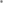
\includegraphics[scale=0.23]{resources/star.png}
\end{frame}

\begin{frame}
  \frametitle{Example}
  \includegraphics[scale=0.23]{resources/frame.png}
\end{frame}

\begin{frame}
  \frametitle{Our work}

  \begin{itemize}
  \item Reduce a decidable fragment of SL to a decidable FO theory.
  \item Fits into the SMT framework.
  \item Satisfiability, entailment, frame inference, and abduction problems for SL using SMT solvers.
  \item Combining SL with other theories.
  \item Implemented in the GRASShopper tool.
  \end{itemize}

\end{frame}

\section{Theoretical results}

\begin{frame}
  \frametitle{Decidable SL fragment: \JoshLogic}

\JoshLogicSimple (separation logic formulas for linked lists) introduced in \cite{BerdineETAL04DecidableFragmentSeparationLogic}.

\vspace{2ex}

\JoshLogicSimple
\begin{equation*}
  \Sigma ::= x = y \mid x \neq y \mid x \mapsto y \mid \liste{x}{y} \mid \Sigma * \Sigma
\end{equation*}
%$x,y \in \vars$

\vspace{2ex}

With extend \JoshLogicSimple to \JoshLogicSimple by adding boolean connective on top:
\begin{equation*}
  H ::= \Sigma \mid \neg H \mid H \land H
\end{equation*}

\end{frame}

\begin{frame}
  \frametitle{Semantics of \JoshLogic (1)}

$\tightmodelsStandard{H}$ \\
$A$: heap interpretation (total)\\
$X$: subset of $A$ over which the formula is interpreted (footprint)

\vspace{1ex}

{\small
\begin{align*}
 & \tightmodelsStandard{x = y}&
\text{iff  }& x^\alg = y^\alg \text{ and } X^\alg = \emptyset\\
 & \tightmodelsStandard{x \neq y}&
\text{iff  }& x^\alg \neq y^\alg \text{ and } X^\alg = \emptyset\\
 &\tightmodelsStandard{x \mapsto y}&
\text{iff  }&  \edge^\alg(x^\alg) = y^\alg \text{ and } X^\alg = \{x^\alg\}\\
 & & & & \\
 &\tightmodelsStandard{H_1 * H_2}&
\text{iff  }& \exists U_1, U_2.\, U_1\!\cup\!U_2 = X^\alg \text{ and } U_1\!\cap\!U_2 = \emptyset \text{ and} \\
  &  &  & \tightmodels{\alg[X \mapsto U_1]}{X}{H_1} \text{ and } \tightmodels{\alg[X \mapsto U_2]}{X}{H_2} \\ 
\end{align*}
}

\end{frame}

\begin{frame}
  \frametitle{Semantics of \JoshLogic (2)}

{\small
\begin{align*}
 &\tightmodelsStandard{\liste{x}{y}}&
\text{iff  }& \exists n \ge 0. \ \tightmodelsStandard{\listen{x}{y}{n}} \\
 &\tightmodelsStandard{\listen{x}{y}{0}}&
\text{iff  }& x^\alg = y^\alg \text{ and } X^\alg = \emptyset \\
 &\tightmodelsStandard{\listen{x}{y}{n+1}}&
\text{iff  }& \exists u \in \nodesort^\alg. \ \tightmodels{\alg[z \mapsto u]}{X}{x \mapsto z * \listen{z}{y}{n}} \\
  &  &  & \text{ and } x^\alg \neq y^\alg \text{ and } z \neq x \text{ and } z \neq y \\
 & & & & \\
 &\tightmodelsStandard{H_1 \land H_2}&
\text{iff  }&  \tightmodelsStandard{H_1} \text{ and } \tightmodelsStandard{H_2} \\
 &\tightmodelsStandard{\neg H}&
\text{iff  }&  \text{not } \tightmodelsStandard{H}
\end{align*}
}

\end{frame}

\begin{frame}
  \frametitle{\LRJQ: graph reachability and stratified sets}

\begin{equation*}
\begin{array}{rcl}
  & & \text{graph reachability} \\
  T & ::= & x \mid \edge(T) \\
  A & ::= & T = T \mid \creach{T}{T}{T} \\
  R & ::= & A \mid \neg R \mid R \land R \mid R \lor R \\
   & & \\
  & & \text{stratified sets} \\
  S & ::= & X \mid \emptyset \mid S \setminus S \mid S \cap S \mid S \cup S \mid \cset{x}{R} \quad \text{$x$ not below $h$ in $R$} \\
  B & ::= & S = S \mid T \in S \\
   & & \\
  & & \text{top level boolean combination} \\
  F & ::= & A \mid B \mid \lnot F \mid F \land F \mid F \lor F 
  \end{array} 
\end{equation*}

\end{frame}

\begin{frame}
  \frametitle{\LRJQ}
    The theory $\lrjqtheory$ is the disjoint combination of:
    \begin{itemize}
    \item a theory of reachability in function graphs $\graphtheory$
    \begin{itemize}
    \item types: $\set{\nodesort}$
    \item function symbols $\set{h}$
    \item predicate symbols $\set{\reachsym}$
    \end{itemize}
    \item a theory of stratified sets $\settheory$~\cite{Zarba04CombiningSetsElements}
    \begin{itemize}
    \item types: $\set{\nodesort, \setsort}$
    \item function symbols $\set{\emptyset, \cap, \cup, \setminus}$
    \item predicate symbols $\set{\in}$
    \end{itemize}
    \end{itemize}

\end{frame}

\begin{frame}
  \frametitle{$\graphtheory$: theory of function graphs}

  What is a function graph ?\\
  A graph where each node has one outgoing edge (per function).

  \vspace{1ex}

  Why a graph and not just functions ?\\
  Rather than just the successors we are interested of in paths (transitive closure of the functions).
  
  \vspace{1ex}
  
  $\creach{t_1}{t_2}{t_3}$ is true if there exists a path in the graph of $h$ that connects $t_1$ and $t_2$ without going through $t_3$.
  
  \vspace{1ex}
  
  $\ls(x,y)$ is a shortcut for $\creach{x}{y}{y}$

  $\Btwn(x,y)$ is a shortcut for $\{z. \creach{x}{z}{y} \land z \neq y\}$

\end{frame}

\begin{frame}
  \frametitle{$\graphtheory$: examples}
  \includegraphics[scale=0.25]{reach.png}
\end{frame}

\subsection{$\text{SLL}\mathbb{B}$ to GRASS}

\begin{frame}
  \frametitle{\JoshLogic $\quad \rightarrow \quad$ \LRJQ (1)}

  Usual way of translating SL to FO:
  \begin{itemize}
  \item structure: uses $\graphtheory$ to encode the shape of the heap (pointers)
  \item footprint: uses $\settheory$ to encode the part of the heap used by a formula
  \end{itemize}

  \vspace{2ex}

  Negation $\Rightarrow$ things get more complicated 
  \begin{itemize}
  \item structure: uses $\graphtheory$ and $\settheory$ to encode the shape of the heap (pointers) and disjointness
  \item set definition: uses $\settheory$ for keep track of the sets that will make the footprint
  \end{itemize}

\end{frame}

\begin{frame}
  \frametitle{\JoshLogic $\ \rightarrow \ $ \LRJQ : ~ $*$ or below}
  \begin{align*}
    \str{Y}{x = y} = {} & (x = y,\; Y = \emptyset) \\
    %
    \str{Y}{x \neq y} = {} & (x \neq y,\; Y = \emptyset) \\[1ex]
    %
    \str{Y}{x \mapsto y} = {} & (\edge(x)=y,\; Y = \{x\})\\[1ex]
    %
    \str{Y}{\ls(x,y)} = {} & (\reach{x}{y},\;  Y = \Btwn(x,y)) \\[1ex]
    %
    \str{Y}{\Sigma_1 * \Sigma_2} = {} &
    \text{let } \text{$Y_1,Y_2 \in \vars$ fresh } \\
    & \text{ and } (F_1,G_1) = \tr_{Y_1}(\Sigma_1) \\
    & \text{ and } (F_2,G_2) = \tr_{Y_2}(\Sigma_2)\\
    & \text{in } (F_1 \land F_2 \land Y_1\!\cap\!Y_2\!=\!\emptyset,\;     Y\!=\!Y_1\!\cup\!Y_2 \land G_1 \land G_2)\\
  \end{align*}
\end{frame}

\begin{frame}
  \frametitle{\JoshLogic $\ \rightarrow \ $ \LRJQ : ~ boolean structure}
  \begin{align*}
    \tr_X(\Sigma) = {} & \text{let } \text{$Y \in \vars$ fresh and } (F,G) = \str{Y}{\Sigma} \\
    & \text{ in }(F \land X\!=\!Y,\; G)\\[1ex]
    %
    \tr_X(\neg H) = {} &
    \letin{(F,G)}{\tr_{X}(H)} \; (\neg F,\; G)\\[1ex]
    %
    \tr_X(H_1\!\land\!H_2) = {} &
    \text{let } (F_1,G_1) = \tr_X(H_1) \text{ and }
    (F_2,G_2) = \tr_X(H_2) \\
    & \text{in }(F_1 \land F_2,\; G_1 \land G_2)\\[1ex]
    %
    \trfull{H}{X} = {} & \letin{(F,G)}{\tr_X(H)} \; F \land G
  \end{align*}%
\end{frame}

\begin{frame}
  \frametitle{Example: without negation}
a non-empty acyclic list segment from $x$ to $z$
\[ \alert<2>{x \neq z} \alert<5>{*} \alert<3>{x \mapsto y} \alert<6>{*} \alert<4>{\liste{y}{z}} \]

translate to
\[
\begin{array}{l}
\alert<2>{x \neq z} \land
\alert<3>{\edge(x)=y} \land
\alert<4>{\reach{y}{z}} \land
\alert<5>{Y_2\!\cap\!Y_3 = \emptyset} \land
\alert<6>{Y_4\!\cap\!Y_5 = \emptyset} \land
\alert<7>{X = Y_1} \land {} \\
\alert<5>{Y_1\!=\!Y_2\!\cup\!Y_3} \land
\alert<2>{Y_2\!=\!\emptyset} \land
\alert<6>{Y_3\!=\!Y_4\!\cup\!Y_5} \land %{} \\
\alert<3>{Y_4\!=\!\{x\}} \land
\alert<4>{Y_5\!=\!\Btwn(y,z)}
\end{array}
\]
\end{frame}

\begin{frame}
  \frametitle{Example: with negation}
a non-empty acyclic list segment from $x$ to $z$
\[ \alert<2>{\neg} ( \alert<1>{x \neq z* x \mapsto y * \liste{y}{z}} ) \]

\alt<1>{ignoring the negation (same as before):}{with negation (only the structure part is changed)}
\[
\begin{array}{l}
\text{structure}\\
\alt<1>{
x \neq z \land \edge(x)=y \land \reach{y}{z} \land
Y_2\!\cap\!Y_3 = \emptyset \land
Y_4\!\cap\!Y_5 = \emptyset \land
X = Y_1
}{
x = z \lor \edge(x) \neq y \lor \neg\reach{y}{z} \lor
Y_2\!\cap\!Y_3 \neq \emptyset \lor
Y_4\!\cap\!Y_5 \neq \emptyset \lor
X \neq Y_1
}\\[1ex]

\text{set definitions}\\
Y_1\!=\!Y_2\!\cup\!Y_3 \land
Y_2\!=\!\emptyset \land
Y_3\!=\!Y_4\!\cup\!Y_5 \land %{} \\
Y_4\!=\!\{x\} \land
Y_5\!=\!\Btwn(y,z)
\end{array}
\]
\end{frame}

\begin{frame}
  \frametitle{Why is that correct ?}
    
Translation: $\trfull{H}{X} = \ \letin{(F,G)}{\tr_X(H)} \; F \land G$

\vspace{1ex}

% stratified sets has existentially quantified set variables
the auxiliary variables $Y_i$ (in $G$) are existentially quantified

\vspace{1ex}

% when taking negation we should get some forall (which is very bad)
below negation, the existential quantifiers should become universal

\pause{}
\vspace{1ex}

% therefore \exists and \forall are the same if we can preserve the definitions
the $Y_i$ are defined as finite unions of set comprehensions\\
$\rightarrow$ satisfiable in any given heap interpretation $\alg$

\pause{}
\vspace{1ex}

% observation: in \JoshLogic the footprint is uniquely defined by the formula (TODO modulo partial interpretation / models)
Due to the precise semantics of \JoshLogic\\
$\rightarrow$ \alert{exists exactly one assignment of the $Y_i$} that makes $G$ true in $\alg$

\pause{}
\vspace{1ex}

$\exists Y_1,\dots,Y_n.\, F \land G$ \ \  and\\
$\forall Y_1,\dots,Y_n.\, G \Rightarrow F$ \ are equivalent. 

\end{frame}

\begin{frame}
  \frametitle{Decision procedure for \LRJQ: $\settheory$}
    \begin{enumerate}
    \item Transform $F$ in nnf and eliminate all $S_1 \neq S_2$:
    \[S_1 \neq S_2 \; \leadsto \; x \in S_1 \setminus S_2 \cup S_2 \setminus S_1 \qquad \text{where $x \in \vars$ fresh}\]

    \item Eliminate all set comprehensions by applying:
      \[C[\cset{x}{R}] \; \leadsto \; C[X] \land (\forall x.\, x \in X \Leftrightarrow R) \qquad \text{where $X \in \vars$ fresh}\]

    \item Instantiate all universal quantifiers as follows. Let $t_1,\dots,t_n$ be the terms of sort $\nodesort$ that do not contain quantified variables. Then apply:
    \[(\forall x.\, x \in X \Leftrightarrow R) \; \leadsto \; (t_1 \in X \Leftrightarrow R[t_1/x]) \land \ldots \land  (t_n \in X \Leftrightarrow R[t_n/x])\]
    \end{enumerate}
    This result is a quantifier-free $\lrjqsig$-formula.
\end{frame}

\begin{frame}
  \frametitle{Decision procedure for \LRJQ: set reduction example (1)}

Consider the \LRJQ formula (unsat):
\[F \equiv \cset{x}{\reach{x}{y}} = \univset \land \reach{y}{z} \land \neg (\reach{w}{z})\]
After rewriting set operation:
{\small
\[
F_2 \equiv S = U \land \reach{y}{z} \land \neg (\reach{w}{z}) \land (\forall x.\, x \in S \Leftrightarrow \reach{x}{y}) \land (\forall x.\, x \in U \Leftrightarrow x = x)
\]
}
After instantiating the quantifiers:
\begin{align*}
G \equiv {} & S = 
U \land \reach{y}{z} \land \neg (\reach{w}{z}) \land {} \\
& (y \in S \Leftrightarrow \reach{y}{y}) \land (z \in S \Leftrightarrow \reach{z}{y}) \land (w \in S \Leftrightarrow \reach{w}{y}) \land {} \\
& (y \in U \Leftrightarrow y = y) \land (z \in U \Leftrightarrow z = z) \land (w \in U \Leftrightarrow w = w)
\end{align*}
\end{frame}

\begin{frame}
  \frametitle{Decision procedure for \LRJQ: set reduction example (2)}
After instantiating the quantifiers:
\begin{align*}
G \equiv {} & S = 
U \land \reach{y}{z} \land \neg (\reach{w}{z}) \land {} \\
& (y \in S \Leftrightarrow \reach{y}{y}) \land (z \in S \Leftrightarrow \reach{z}{y}) \land (w \in S \Leftrightarrow \reach{w}{y}) \land {} \\
& (y \in U \Leftrightarrow y = y) \land (z \in U \Leftrightarrow z = z) \land (w \in U \Leftrightarrow w = w)
\end{align*}
To see that this formula is unsatisfiable in $\lrjqtheory$, we simplify $G$ to the equivalent formula:
\begin{align*}
G' \equiv {} & \alert{S = U} \land \alert{\reach{y}{z}} \land \alert{\neg (\reach{w}{z})} \land y \in U \land z \in U \land \alert{w \in U} \land {}\\
& (y \in S \Leftrightarrow \reach{y}{y}) \land (z \in S \Leftrightarrow \reach{z}{y}) \land \alert{(w \in S \Leftrightarrow \reach{w}{y})}
\end{align*}

\end{frame}

\begin{frame}
  \frametitle{Decision procedure for \LRJQ: $\graphtheory$}
  
  By \cite{TotlaWies13CompleteInsterpolation} we know $\graphtheory$ is a local theory extensions \cite{SofronieStokkermans05HierarchicReasoninginLocalTheoryExtensions}.
  We just need to instantiate a set of axioms on the ground terms in the formula.

{\scriptsize
  \begin{align*}
    \textsf{Reflexive } & \creach{x}{x}{u}\\
    \textsf{Step } & \creach{x}{h(x)}{u} \lor x = u\\
    \textsf{SelfLoop } & h(x)=x \land \reach{x}{y} \mimplies x = y\\
    \textsf{Sandwich } & \creach{x}{y}{x} \mimplies x = y\\
    \textsf{Reach } & \creach{x}{y}{u} \mimplies \reach{x}{y}\\
    \textsf{Linear1 } & \reach{x}{y} \mimplies \creach{x}{u}{y} \lor \creach{x}{y}{u}\\
    \textsf{Linear2 } & \creach{x}{y}{u} \land \creach{x}{z}{v} \mimplies \creach{x}{z}{u} \land \creach{z}{y}{u} \lor \creach{x}{y}{v} \land \creach{y}{z}{v} \\
    \textsf{Transitive1 } & \creach{x}{y}{u} \land \creach{y}{z}{u} \mimplies     \creach{x}{z}{u}\\
    \textsf{Transitive2 } & \creach{x}{y}{z} \land \creach{y}{u}{z} \land \reach{y}{z} \mimplies    \creach{x}{y}{u}
  \end{align*}
}

\end{frame}

\begin{frame}
  \frametitle{Decision procedure for \LRJQ: $\graphtheory$}
  \includegraphics[scale=0.22]{resources/partial.png}
\end{frame}

\subsection{And back}

\begin{frame}
  \frametitle{Where are we now ?}
  With the \JoshLogic to \LRJQ translation we can
  \begin{itemize}
  \item Check for satisfiability
  \item Check entailment (reduces to satisfiability of $H_1 \land \neg H_2$)
  \end{itemize}

  \vspace{2ex}

  For the (anti-)frame inference:\\
  finding $F$ in $A \tightentails B*F$ (frame) or $A*F \tightentails B$(antiframe)\\
  we need the inverse translation
\end{frame}

\begin{frame}
  \frametitle{\LRJQ $\ \rightarrow \ $ \JoshLogic}

  Requirements:
  \begin{itemize}
  \item a \LRJQ formula $F$ obtained from a \JoshLogic formula (for the sake of simplicity)
  \item a model generating SMT solver (e.g. \zthree),
  \end{itemize}

  Steps:
  \begin{itemize}
  \item get for all the partial interpretations that satisfy $F$
  \item for all a partial interpretation:
  \begin{itemize}
  \item construct $\hsucc: \nodesort \pto \nodesort$
  \item extract the \emph{pure} part from the interpretation
  \item lift the interpretation to SL using $h$ and $\hsucc$.
  \end{itemize}
  \end{itemize}
  where $\hsucc$ is the closest successor node in the partial interpretation

\end{frame}

\begin{frame}
  \frametitle{\LRJQ $\ \rightarrow \ $ \JoshLogic: example }

$\ldots$\\
assume($\ls(x,z)$);\\
if ($x \neq z$)\\
\mbox{} ~~~~ free\_head($x$); //frame with precondition $x\mapsto y$\\
$\ldots$\\

\vspace{1ex}

\LRJQ:
{\small $x \neq z \land \reach{x}{z} \land \edge(x)\!=\!y \land  X\!=\!\Btwn(x,z) \land Y\!=\!\set{x} \land Z\!=\!X \setminus Y$}
  
\pause{}
\vspace{.5ex}

Partial interpretations:
\begin{minipage}{0.5\linewidth}
  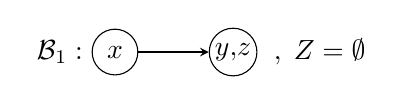
\begin{tikzpicture}
  \node (a) at (-.7,0) {$\oalg_1:$};
  \node[draw,circle] (x) at (0,0) {$x$};
  \node[draw,circle,inner sep=1pt] (y) at (1.5,0) {$y,\!z$};
  \node (Z) at (2.6,0) {$, \; Z = \emptyset$};
  % \node (yd) at (2,-.5) {\tiny$\emptyset$};
  \path[-stealth] (x) edge (y);
  \end{tikzpicture}\\[.5ex]
  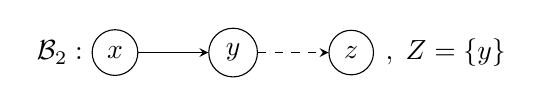
\begin{tikzpicture}
  \node (a1) at (4,0) {$\oalg_2:$};
  \node[draw,circle] (x1) at (4.7,0) {$x$};
  \node (Z1) at (8.9,0) {$, \; Z = \set{y}$};
  \node[draw,circle] (y1) at (6.2,0) {$y$};
  \node[draw,circle] (z1) at (7.7,0) {$z$};
  \path[-stealth] (x1) edge (y1);
  \path[-stealth,dashed] (y1) edge (z1);
  \end{tikzpicture}
\end{minipage}

\pause{}
\vspace{1ex}
$\itr_Z(\oalg_1)= x\!\neq\!z * x\!\neq\!y * y\!=\!z$\\
$\itr_Z(\oalg_2) = x\!\neq\!z * x\!\neq\!y * y\!\neq\!z * \ls(y,z)$\\[1ex]
$\itrfull_Z(F) = \itr_Z(\oalg_1) \lor \itr_Z(\oalg_2) \equiv x\!\neq\!z * x\!\neq\!y * \ls(y,z)$.

\end{frame}

\begin{frame}
  \frametitle{Combination with other theories and extensions}
  \begin{itemize}
  \item The theories $\graphtheory$ and $\settheory$ are stably infinite with respect to sort $\nodesort$. (Nelson-Oppen)

  \item More pointers: we can extend the signature with $\fldsort$ and uses $\reachsymf$ with different fields.
  We can the also do read and write on the fields (array theory).

  \item Data: we can add data and constraints if it is local. 

{\scriptsize
$\str{Y}{\mathsf{sls}(x,y)} = (\reachf{\mathit{h}}{x}{y} \land \forall z, w \in Y.\, \reachf{\mathit{h}}{z}{w} \Rightarrow \mathit{d}(z)\! \leq\! \mathit{d}(w), \; Y\!=\!\Btwn(x,y))$
}
  \item More complex data structures, e.g. doubly linked lists

{\scriptsize
$
\begin{array}{l}
\str{Y}{\mathsf{dlls}(x,a,y,b)} =
 ( \begin{array}[t]{l}
  \reachf{n}{x}{y} \land (x\!=\!y \land a\!=\!b \lor   p(x)\!=\!a \land n(b)\!=\!y \land b \in Y) \land {} \\
\forall z \in Y.\, n(z) \in Y \Rightarrow p(n(z))\!=\!z, \;
Y\!=\!\Btwn(x,y) \; )
\end{array}
\end{array}
$
}

  We are also considering implementing a decision procedure for trees.
 
  \end{itemize}
\end{frame}

\section{Implementation}
\subsection{\Tool}

\begin{frame}
  \frametitle{Reduction steps}

  We have implemented the translation is \Tool.

  \vspace{1ex}

  Takes as input a program with \JoshLogic specification and\\
  reduces it to a program with FO specification (Boogie-like)

  \vspace{1ex}
  The reduction is as follows:
  \begin{enumerate}
  \item if as choose + assume
  \item replace loops by tail-recursive method
  \item \JoshLogic $\rightarrow$ \LRJQ, adding the heap (frame, memory accesses)
  \item SSA, add assert/assume at call site
  \end{enumerate}

  \vspace{2ex}

  Let's look at a concrete example: merge sort.
\end{frame}

\subsection{Implicit frame inference}

\begin{frame}
  \frametitle{Frame inference}

  Reconstructing the frame from the partial interpretations does not work (exponential in the works case).

  \vspace{1ex}
  
  Can we avoid the explicit computation of the frame ?\\
  (e.g. have an axiomatic definition of the frame rule)

  \vspace{1ex}

  In previous example we had:
  \begin{center}
  \texttt{assume Frame(Alloc\_1, Alloc\_2, next, next\_1);}
  \end{center}

\end{frame}

\begin{frame}
  \frametitle{\texttt{assume Frame(Alloc\_1, Alloc\_2, next, next\_1);}}

Meaning: a path which doesn't go through the frame is unchanged.

\vspace{2ex}

For this we need the entry point of $x$ in the set $X$ by following $\edge$,\\
denoted by $\ep_{X,\edge}(x)$

\vspace{2ex}

$\mkframe(X,A,\edge,\edge') =$
\[
\begin{array}[t]{l}
\forall x. \, x \in A \setminus X \Rightarrow \sel(\edge', x) = \sel(\edge, x) \land {} \\
\forall x\, y \, z. \, \creachf{\edge}{x}{y}{\ep_{X,\edge}(x)} \Rightarrow (\creachf{\edge}{x}{y}{z} \Leftrightarrow \creachf{\edge'}{x}{y}{z}) \land {}\\
\forall x\, y\, z. \, x \in A \setminus X \land \ep_{X,\edge}(x)=x \Rightarrow (\creachf{\edge}{x}{y}{z} \Leftrightarrow \creachf{\edge'}{x}{y}{z})
\end{array}
\]
\end{frame}

\begin{frame}
  \frametitle{$\ep_{X,\edge}(x)$}
  
  Axioms defining the entry point function:
  \begin{align*}
    & \forall x. \, \reachf{\edge}{x}{\ep_{X,\edge}(x)} \\[.5em]
    & \forall x. \, \ep_{X,\edge}(x) \in X \lor \ep_{X,\edge}(x) =     x\\
    & \forall x \, y. \, \reachf{\edge}{x}{y} \land y \in X     \Rightarrow \ep_{X,\edge}(x) \in X \land     \creachf{\edge}{x}{\ep_{X,\edge}(x)}{y}
  \end{align*}
  $\ep{X,\edge}$ is local (idempotent), we can use the same approach as $\graphtheory$.

  %TODO picture

\end{frame}

\begin{frame}
  \frametitle{$\ep$}
  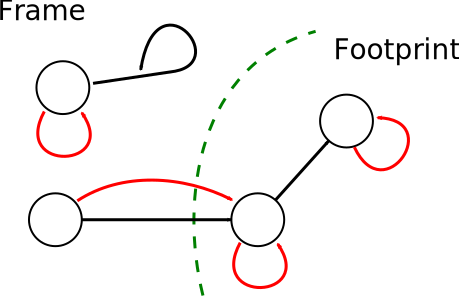
\includegraphics[scale=0.22]{resources/ep.png}
\end{frame}


\subsection{Experimental results}

\begin{frame}
  \frametitle{experiments}
\begin{table}[t]%{l}{5cm}
{\tiny
\centering
%\begin{minipage}{.\linewidth}
\renewcommand{\tabcolsep}{0.14cm}
\begin{tabular}{|l|c|c|c|c|c|c|c|c||l|c|c|c|c|c|c|c|c|}
\hline
program & \multicolumn{2}{|c|}{sl} & \multicolumn{2}{|c|}{dl} & \multicolumn{2}{|c|}{rec sl} & \multicolumn{2}{|c||}{sls} & 

program & \multicolumn{2}{|c|}{sl}  & \multicolumn{2}{|c|}{dl} & \multicolumn{2}{|c|}{rec sl} & \multicolumn{2}{|c|}{sls}
\\

\cline{2-9}
\cline{11-18}
%\hline

& \# & t & \# & t & \# & t & \# & t &
& \# & t & \# & t & \# & t & \# & t \\

\hline
%\hline

concat & 4 & 0.1 & 5 & 1.3 & 6 & 0.6 & 5 & 0.2 & 
insert & 6 & 0.2 & 5 & 1.5 & 5 & 0.2 & 6 & 0.4 \\

%\hline

copy    & 4 & 0.2 & 4 & 3.9 & 6 & 0.8 & 7 & 3.5 & 
reverse & 4 & 0.1 & 4 & 0.5 & 6 & 0.2 & 4 & 0.2 \\

%\hline

filter & 7 & 0.6 & 5 & 1.1 & 8 & 0.4 & 5 & 1.1 & 
remove & 8 & 0.2 & 8 & 0.8 & 7 & 0.2 & 7 & 0.5 \\

%\hline

free     & 5 & 0.1 & 5 & 0.3 & 4 & 0.1 & 5 & 0.1 & 
traverse & 4 & 0.1 & 5 & 0.3 & 3 & 0.1 & 4 & 0.2 \\

\cline{2-7}
\cline{11-16}

%\hline

\multicolumn{7}{|l|}{insertion sort} & 10 & 0.7 &
\multicolumn{7}{|l|}{double all} & 7 & 2.2\\

\multicolumn{7}{|l|}{merge sort} & 25 & 24 &
\multicolumn{7}{|l|}{pairwise sum} & 10 & 20 \\
\hline
\end{tabular}
}
\end{table}

\begin{description}
\item[sl] singly-linked list (loop or recursion)
\item[dl] doubly-linked list
\item[sls] sorted lists
\end{description}
\begin{description}
\item[\#] number of VCs
\item[t] total time in second
\end{description}
\end{frame}

\section*{Conclusion}

\begin{frame}
  \frametitle{Related work}
{\small
  \begin{itemize}
  \item Most prominent decidable fragments of SL: linked lists~\cite{BerdineETAL04DecidableFragmentSeparationLogic}, decidable in polynomial time~\cite{CooketALFragmentSepLog} (graph-based).

\item SL $\rightarrow$ FO: \cite{Calcagno05fromseparation} (no inductive predicate) and~\cite{bobot12icfem} (not a decidable fragment).
%Neither of these approaches considers frame inference, abduction, or theory combination.
%More recently and concurrently to us, they have also considered the problem of theory combination~\cite{PerezR13}. The authors of~\cite{DBLP:conf/atva/BouajjaniDES12} describe another hybrid approach in which an SL decision procedure for entailment is extended to enable reasoning about quantified constraints on data. However, \cite{DBLP:conf/atva/BouajjaniDES12} does not address theory combination in general. Also, neither~\cite{DBLP:conf/pldi/PerezR11} nor~\cite{DBLP:conf/atva/BouajjaniDES12} consider frame inference or abduction.

\item Alternatives to SL: (implicit) dynamic frames~\cite{DBLP:journals/fac/Kassios11} and region logic~\cite{DBLP:conf/ecoop/BanerjeeNR08,DBLP:conf/vmcai/RosenbergBN12}.
\item The connection between SL and implicit dynamic frames has been studied in~\cite{DBLP:journals/corr/abs-1203-6859}.

\item SMT-based decision procedures for theories of reachability in graphs~\cite{DBLP:conf/popl/LahiriQ08, WiesMK11, TotlaWies13CompleteInsterpolation}
, decision procedures for theories of stratified sets~\cite{Zarba04CombiningSetsElements}.

\end{itemize}
}
\end{frame}

\begin{frame}
  \frametitle{Work in progress, future work}

  \begin{itemize}
  \item dealing with the frame (still work in progress)
  \item more example using other theories (arrays, integers, ...)
  \item inferring \LRJQ predicate definition from \JoshLogic definition
  \item decision procedure for trees
  \item abstraction/modularity (generic list)
  \item etc.
  \end{itemize}

\end{frame}

\begin{frame}

  \begin{center}
  \huge
  Questions ?
  \end{center}
\end{frame}

\begin{frame}[allowframebreaks]{References}
  {\tiny
  %\bibliographystyle{annotate}
  %\bibliographystyle{plainnat}
  \bibliographystyle{cell}
  %\bibliographystyle{abbrvnat}
  \bibliography{biblio}
  }
\end{frame}

\end{document}
